% CS301 Computer Networks -- Mini-Project Progress Report
% Layout cloned from the CS255 FEC report (Sem IV). Edit the macros below first.
\documentclass[11pt,a4paper]{article}

% ---------------------------------------------------------------- report metadata
\newcommand{\CourseLine}{CS301 --- Computer Networks}
\newcommand{\ReportLine}{Mini-Project Progress Report -- I}
\newcommand{\HeaderLeft}{CS301 Mini-Project Progress Report -- I}
\newcommand{\HeaderRight}{241CS257 \textbar{} Somyak Priyadarshi Mohanta}
\newcommand{\RepoName}{somyaknotfound/cn\_project}
\newcommand{\RepoURL}{https://github.com/somyaknotfound/cn_project}

% ---------------------------------------------------------------- packages
\usepackage[utf8]{inputenc}
\usepackage[T1]{fontenc}
\usepackage[margin=1in]{geometry}
\usepackage{setspace}
\usepackage{amsmath,amssymb}
\usepackage{graphicx}
\usepackage{booktabs}
\usepackage{array}
\usepackage{multirow}
\usepackage{tabularx}
\usepackage[table]{xcolor}
\usepackage{enumitem}
\usepackage{titlesec}
\usepackage{fancyhdr}
\usepackage{caption}
\usepackage{float}
\usepackage{algorithm}
\usepackage{algpseudocode}
\usepackage{tikz}
\usetikzlibrary{positioning,arrows.meta,shapes.geometric,fit,calc}
\usepackage{dirtree}
\usepackage{hyperref}

\hypersetup{
  colorlinks=true,
  linkcolor=blue!70!black,
  citecolor=blue!70!black,
  urlcolor=blue!80!black,
  pdftitle={\HeaderLeft},
}

% ---------------------------------------------------------------- spacing
\setstretch{1.25}
\setlength{\parindent}{0pt}
\setlength{\parskip}{6pt}
\renewcommand{\arraystretch}{1.45}

% ---------------------------------------------------------------- headings: "1. Title" with rule, "1.1. Title", italic "1.1.1. Title"
\titleformat{\section}{\Large\bfseries}{\thesection.}{0.5em}{}[\vspace{-0.5ex}\titlerule]
\titleformat{\subsection}{\large\bfseries}{\thesubsection.}{0.5em}{}
\titleformat{\subsubsection}{\normalsize\itshape}{\thesubsubsection.}{0.5em}{}
\titlespacing*{\section}{0pt}{3ex plus 1ex}{1.5ex}
\titlespacing*{\subsection}{0pt}{2.5ex plus 1ex}{1ex}
\titlespacing*{\subsubsection}{0pt}{2ex plus 1ex}{0.8ex}

% ---------------------------------------------------------------- header / footer
\pagestyle{fancy}
\fancyhf{}
\fancyhead[L]{\HeaderLeft}
\fancyhead[R]{\HeaderRight}
\fancyfoot[C]{\thepage}
\renewcommand{\headrulewidth}{0.4pt}
\setlength{\headheight}{14pt}

% ---------------------------------------------------------------- captions, lists
\captionsetup{font=normalsize, labelsep=colon, skip=6pt}
\captionsetup[table]{position=top}
\setlist[enumerate]{leftmargin=*, itemsep=2pt}
\setlist[itemize]{leftmargin=*, itemsep=2pt}

% ---------------------------------------------------------------- house macros
\newcommand{\pros}{\textcolor{green!50!black}{\textbf{Pros:}}~}
\newcommand{\cons}{\textcolor{red!70!black}{\textbf{Cons:}}~}
\newcommand{\todo}[1]{\textcolor{red}{\textbf{[TODO: #1]}}}
\newcommand{\code}[1]{\texttt{#1}}

% pastel boxes used in every TikZ figure
\tikzset{
  box/.style={draw=black!60, rounded corners=2pt, align=center, inner sep=4pt, minimum height=1.0cm},
  redbox/.style={box, fill=red!8},
  orangebox/.style={box, fill=orange!10},
  yellowbox/.style={box, fill=yellow!18},
  greenbox/.style={box, fill=green!10},
  bluebox/.style={box, fill=blue!8},
  graybox/.style={box, fill=black!5},
  pinkbox/.style={box, fill=magenta!8},
  arr/.style={-{Stealth[length=2mm]}, thick},
}

\begin{document}

% ================================================================ TITLE PAGE
\hypersetup{pageanchor=false}
\begin{titlepage}
\centering
\vspace*{0.6cm}
{\large\bfseries National Institute of Technology Karnataka, Surathkal\par}
\vspace{6pt}
{\large\bfseries Department of Computer Science and Engineering\par}
\vspace{18pt}
{\CourseLine\par}
\vspace{6pt}
{\ReportLine\par}
\vspace{1.4cm}

\rule{\linewidth}{1pt}\par
\vspace{0.35cm}
{\LARGE\bfseries\setstretch{1.55}
Threshold-Aware Similarity Caching\\
for Named Data Networks:\\
Bounding Retry Delay\\
under Congestion using ns-3\par}
\vspace{0.25cm}
\rule{\linewidth}{1pt}\par

\vspace{1.0cm}
{\bfseries Project Repository\par}
\vspace{6pt}
\href{\RepoURL}{\small\texttt{\RepoName}}\par

\vspace{1.0cm}
\begin{tabular}{@{}r@{\hspace{8pt}}l@{}}
  \textbf{Students:} & Somyak Priyadarshi Mohanta (241CS257) \\[-4pt]
                     & Pranav Shaji (241CSXXX) \\[-4pt]
                     & Chris Tony (241CSXXX) \\[4pt]
  \textbf{Department:} & Computer Science and Engineering \\[-4pt]
  \textbf{Institute:}  & National Institute of Technology Karnataka, Surathkal \\
\end{tabular}

\vspace{0.8cm}
\begin{tabular}{@{}r@{\hspace{8pt}}l@{}}
  \textbf{Guide:}      & Prof. B. R. Chandavarkar \\[-4pt]
  \textbf{Department:} & Computer Science and Engineering, NITK \\
\end{tabular}
\vfill
\end{titlepage}
\hypersetup{pageanchor=true}

% ================================================================ ABSTRACT
\setcounter{page}{1}
\begin{abstract}
\setlength{\parindent}{1.5em}
\noindent\todo{Paragraph 1: context --- content caching, similarity caching, and why the
user-perceived delay of serving an \emph{approximate} answer from a nearby cache matters.}

\todo{Paragraph 2: the gap left by the base paper and the proposed solution, the ns-3/ndnSIM
topology, workloads, and the headline numbers.}
\end{abstract}

\vspace{1em}
\noindent\textbf{Keywords:} Similarity Caching, Cache Networks, Information-Centric
Networking, Content Delivery, Network Simulation, ns-3, ndnSIM, \todo{more}.

\newpage
% ================================================================ CONTENTS
{\setlength{\parskip}{0pt}\setstretch{1.15}\tableofcontents}
\newpage

% ================================================================ 1 INTRODUCTION
\section{Introduction}

Content caching places copies of popular objects close to users so that requests are served
in fewer hops, with lower delay and less upstream traffic. Content Delivery Networks (CDN),
Mobile Edge Computing (MEC) caches and the router caches of Information-Centric Networking
(CCN/NDN) all apply this principle~\cite{jacobson2009ccn,zhang2014ndn}. In each of them a
cache answers a request only on an \emph{exact} match of the content identifier.

\emph{Similarity caching}~\cite{falchi2008metric,pandey2009nn} relaxes that rule: on a miss the
cache may return the cached object most similar to the request, trading exactness for
delay~\cite{neglia2022similarity}. Table~\ref{tab:demo} contrasts the two.

\begin{table}[H]
\centering
\caption{Exact Caching vs.\ Similarity Caching}
\label{tab:demo}
\begin{tabular}{@{}lcc@{}}
\toprule
\textbf{Property} & \textbf{Exact Caching} & \textbf{Similarity Caching} \\
\midrule
Response on hit   & Requested object & Requested object \\
Response on miss  & Forward upstream & Most similar cached object (or forward) \\
Answer quality    & Always exact     & Similarity $s \in [0,1]$ \\
Key metric        & Hit ratio        & Delay \emph{and} similarity \\
\bottomrule
\end{tabular}
\end{table}

\subsection{Motivation}
\todo{Why the user-level delay of similarity caching must be measured on a real packet
network, not only computed in closed form.}

\subsection{Problem Statement}
\todo{One paragraph, written last-sem style: ``Given \ldots, design and implement \ldots, and
validate in ns-3.''}

\subsection{Objectives}
\begin{enumerate}[label=\textbf{O\arabic*.}]
  \item \todo{Reproduce the base-paper analysis and validate it in ns-3/ndnSIM.}
  \item \todo{Design the proposed mechanism.}
  \item \todo{Evaluate across topologies, workloads and link conditions.}
\end{enumerate}

\subsection{Organisation of the Report}
Section~\ref{sec:lit} reviews related work. Section~\ref{sec:method} describes the proposed
methodology. Section~\ref{sec:results} presents experimental results.
Section~\ref{sec:conc} concludes with future work.

% ================================================================ 2 LITERATURE REVIEW
\section{Literature Review}\label{sec:lit}

This section reviews \todo{N} categories of related work. Each subsection is followed by a
pros and cons analysis. A consolidated comparison is given in Table~\ref{tab:compare}.

\subsection{Similarity Caching on General Cache Networks (Base Paper)}

Nakamura and Kamiyama~\cite{nakamura2024analysis} model a cache network as a graph
$G=(V,E)$ of cache nodes $V_c$ and origin nodes $V_o$, with request/response routing along a
fixed path $P_{v,c}$ as in CCN/NDN. On a miss, a cache returns its most similar object with
probability $\alpha$ and forwards otherwise. A client that receives an object with
similarity below its threshold $s$ waits $\delta$ and re-requests. The user-level metric is
the \emph{similar-content delivery delay}:
\begin{equation}
  D_{v,c} = \sum_{s} \beta^{(s)}_v \, D^{s(\geq)}_{v,c},
  \qquad
  D^{s(\geq)} = \sum_{n=1}^{\infty} \Delta^{s(\geq)}_n \, R^{s(\geq)}_n ,
\end{equation}
where $\beta^{(s)}_v$ is the client's acceptance distribution over similarity levels,
$\Delta^{s(\geq)}_n = (n-1)(d^{s(<)}+\delta) + d^{s(\geq)}$ is the delay when the $n$-th
attempt succeeds, and $R^{s(\geq)}_n = (1-\rho^{s(\geq)})^{n-1}\rho^{s(\geq)}$ is its
probability.

\pros First closed-form, user-oriented delay metric for similarity caching over a
multi-node path; captures the client's retry behaviour.

\cons Assumes infinite bandwidth, no queuing and no loss; cache contents are a uniform
random subset rather than the output of a replacement policy; a single global $\alpha$; a
five-node tandem topology; evaluated numerically only.

\begin{figure}[H]
\centering
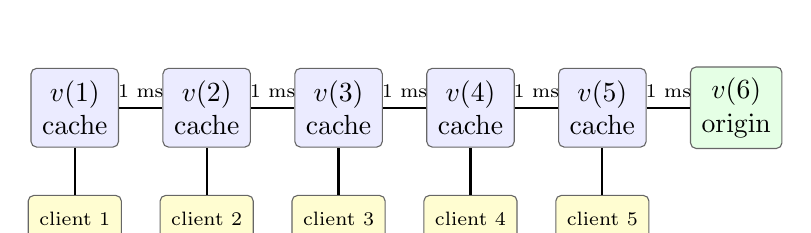
\begin{tikzpicture}[node distance=0.55cm]
  \node[bluebox]  (v1) {$v(1)$\\cache};
  \node[bluebox,  right=of v1] (v2) {$v(2)$\\cache};
  \node[bluebox,  right=of v2] (v3) {$v(3)$\\cache};
  \node[bluebox,  right=of v3] (v4) {$v(4)$\\cache};
  \node[bluebox,  right=of v4] (v5) {$v(5)$\\cache};
  \node[greenbox, right=of v5] (v6) {$v(6)$\\origin};
  \foreach \a/\b in {v1/v2,v2/v3,v3/v4,v4/v5,v5/v6} \draw[thick] (\a) -- node[above]{\scriptsize 1 ms} (\b);
  \foreach \i in {1,...,5} {
    \node[yellowbox, minimum height=0.6cm, below=0.6cm of v\i] (c\i) {\scriptsize client \i};
    \draw[thick] (c\i) -- (v\i);
  }
\end{tikzpicture}
\caption{Tandem topology used in the base paper's numerical evaluation~\cite{nakamura2024analysis}.}
\label{fig:tandem}
\end{figure}

\subsection{\todo{Category B}}
\subsubsection{\todo{Paper}}
\todo{Summary.}

\pros \todo{.}

\cons \todo{.}

\subsection{Comparison of Existing Approaches}

\begin{table}[H]
\centering
\caption{Comparison of Existing Similarity-Caching Approaches}
\label{tab:compare}
\begin{tabular}{@{}p{3.2cm}>{\centering}p{2.2cm}>{\centering}p{2.2cm}>{\centering}p{2.4cm}>{\centering\arraybackslash}p{2.6cm}@{}}
\toprule
\textbf{Approach} & \textbf{Scope} & \textbf{User-Level Metric} & \textbf{Congestion / Loss} & \textbf{Packet-Level Validation} \\
\midrule
Nakamura \& Kamiyama~\cite{nakamura2024analysis} & Network & Yes & No & No \\
\todo{} & & & & \\
\midrule
\textbf{Proposed} & \textbf{Network} & \textbf{Yes} & \textbf{Yes} & \textbf{Yes (ns-3)} \\
\bottomrule
\end{tabular}
\end{table}

\todo{One paragraph naming the gap the table exposes.}

% ================================================================ 3 METHODOLOGY
\section{Proposed Methodology}\label{sec:method}

\subsection{System Overview}
\todo{End-to-end diagram and one-paragraph walkthrough.}

\subsection{ns-3/ndnSIM Simulation Topology}
\todo{Nodes, routers, link delay / bandwidth / qdisc, routing.}

\subsection{Proposed Algorithm}

\begin{algorithm}[H]
\caption{\todo{Name}}
\label{alg:main}
\begin{algorithmic}[1]
\Require Request for object $c$, local cache $\mathcal{B}$, threshold $s$
\Ensure Response object $c'$
\If{$c \in \mathcal{B}$}
  \State \Return $c$ \Comment{\textit{exact hit}}
\EndIf
\State $c' \gets \arg\max_{x \in \mathcal{B}} \mathrm{sim}(c, x)$
\If{\todo{decision rule}}
  \State \Return $c'$ \Comment{\textit{approximate hit}}
\EndIf
\State forward request upstream
\end{algorithmic}
\end{algorithm}

\subsection{Packet / Header Format}

\begin{table}[H]
\centering
\caption{Request Header Format}
\label{tab:header}
\begin{tabular}{@{}lll@{}}
\toprule
\textbf{Field} & \textbf{Width} & \textbf{Description} \\
\midrule
\todo{} & & \\
\bottomrule
\end{tabular}
\end{table}

\subsection{Software Architecture}
\todo{Module table and folder tree.}

\dirtree{%
.1 cn\_project/.
.2 topology/.
.2 cache/.
.2 client/.
.2 experiments/.
.2 analysis/.
}

\subsection{Key Engineering Challenges and Solutions}
\subsubsection{\todo{Challenge}}
\todo{.}

% ================================================================ 4 RESULTS
\section{Results and Analysis}\label{sec:results}

\subsection{Experimental Setup}

\begin{table}[H]
\centering
\caption{Emulation Environment}
\label{tab:setup}
\begin{tabular}{@{}ll@{}}
\toprule
\textbf{Parameter} & \textbf{Value} \\
\midrule
Simulator         & ns-3 with ndnSIM \\
Topology          & \todo{} \\
Link delay / rate & \todo{} \\
Cache size $B$    & \todo{} \\
Catalogue size $C$& \todo{} \\
Trials            & \todo{} \\
\bottomrule
\end{tabular}
\end{table}

\subsection{Performance Metrics}
\begin{itemize}
  \item \textbf{Similar-content delivery delay:} \todo{.}
  \item \textbf{Approximate / exact hit ratio:} \todo{.}
  \item \textbf{Delivered similarity:} \todo{.}
  \item \textbf{Upstream traffic:} \todo{.}
\end{itemize}

\subsection{Validation Against the Analytical Model}
\todo{Simulated vs.\ closed-form delay, base-paper settings.}

% ================================================================ 5 CONCLUSION
\section{Conclusions and Future Work}\label{sec:conc}

\subsection{Summary of Achievements}
\todo{.}

\subsection{Limitations}
\begin{enumerate}
  \item \todo{.}
\end{enumerate}

\subsection{Future Work}
\begin{enumerate}
  \item \todo{.}
\end{enumerate}

% ================================================================ REFERENCES
\begin{thebibliography}{99}

\bibitem{nakamura2024analysis}
R.~Nakamura and N.~Kamiyama, ``Analysis of similarity caching on general cache networks,''
\emph{IEEE Access}, vol.~12, pp.~163338--163348, 2024, doi: 10.1109/ACCESS.2024.3489620.

\bibitem{neglia2022similarity}
G.~Neglia, M.~Garetto, and E.~Leonardi, ``Similarity caching: Theory and algorithms,''
\emph{IEEE/ACM Trans. Netw.}, vol.~30, no.~2, pp.~475--486, 2022.

\bibitem{falchi2008metric}
F.~Falchi, C.~Lucchese, S.~Orlando, R.~Perego, and F.~Rabitti, ``A metric cache for
similarity search,'' in \emph{Proc. ACM Workshop Large-Scale Distrib. Syst. Inf. Retr.},
2008, pp.~43--50.

\bibitem{pandey2009nn}
S.~Pandey, A.~Broder, F.~Chierichetti, V.~Josifovski, R.~Kumar, and S.~Vassilvitskii,
``Nearest-neighbor caching for content-match applications,'' in \emph{Proc. 18th Int. Conf.
World Wide Web}, 2009, pp.~441--450.

\bibitem{jacobson2009ccn}
V.~Jacobson, D.~K.~Smetters, J.~D.~Thornton, M.~F.~Plass, N.~H.~Briggs, and
R.~L.~Braynard, ``Networking named content,'' in \emph{Proc. 5th ACM CoNEXT}, 2009,
pp.~1--12.

\bibitem{zhang2014ndn}
L.~Zhang \emph{et al.}, ``Named data networking,'' \emph{ACM SIGCOMM Comput. Commun.
Rev.}, vol.~44, no.~3, pp.~66--73, 2014.

\end{thebibliography}

\end{document}
